\subsection{Validazione e collaudo}
\label{validazione_e_collaudo}
\textbf{Durata:} dal 2021\_04\_10 al 2021\_05\_09\\
Il periodo di validazione e collaudo inizia appena concluso il precedente e termina con la \glo{\textbf{RA}}.
Le precondizioni sono:
\begin{itemize}
    \item Le postcondizioni del periodo precedente sono state soddisfatte.
\end{itemize}
Le postcondizioni sono:
\begin{itemize}
    \item Aggiornamento e correzione documenti già prodotti;
    \item Esecuzione dei vari test;
    \item Completamento del prodotto in base a quanto discusso durante la \textbf{RQ};
    \item Consegna dei documenti richiesti in entrata alla \textbf{RA};
    \item Ultimata preparazione della presentazione da esporre in sede di revisione.
\end{itemize}
È composto da nove incrementi e una nuova attività:
\begin{itemize}
    \item \textbf{Incremento e verifica dei documenti}: alcuni dei documenti già prodotti vengono migliorati e aggiornati ({\NdP}, {\PdP}, {\Glossario}, {\PdQ}, \textit{Specifica tecnica}, \textit{Manuale utente}); 
    \item \textbf{Incremento e verifica delle attività}: se necessario vengono migliorate le attività di \textbf{Technology Baseline} per quanto riguarda la progettazione ad alto livello, in particolare la \textbf{Product Baseline} riguardo all'aggiunta di design pattern o di diagrammi di classi o di attività; la parte di codifica, in caso non siano stati riscontrati rallentamenti o ritardi nel progetto, potrebbe comprendere l'implementazione di uno o più casi d'uso opzionali;
    \item \textbf{Validazione e collaudo}: realizzazione degli ultimi test, con successivi controlli finali per garantire un buon livello di qualità e correttezza.
\end{itemize}
\newpage
\subsubsection{Diagramma di Gantt: Validazione e collaudo}
\begin{figure}[ht]
    \centering
    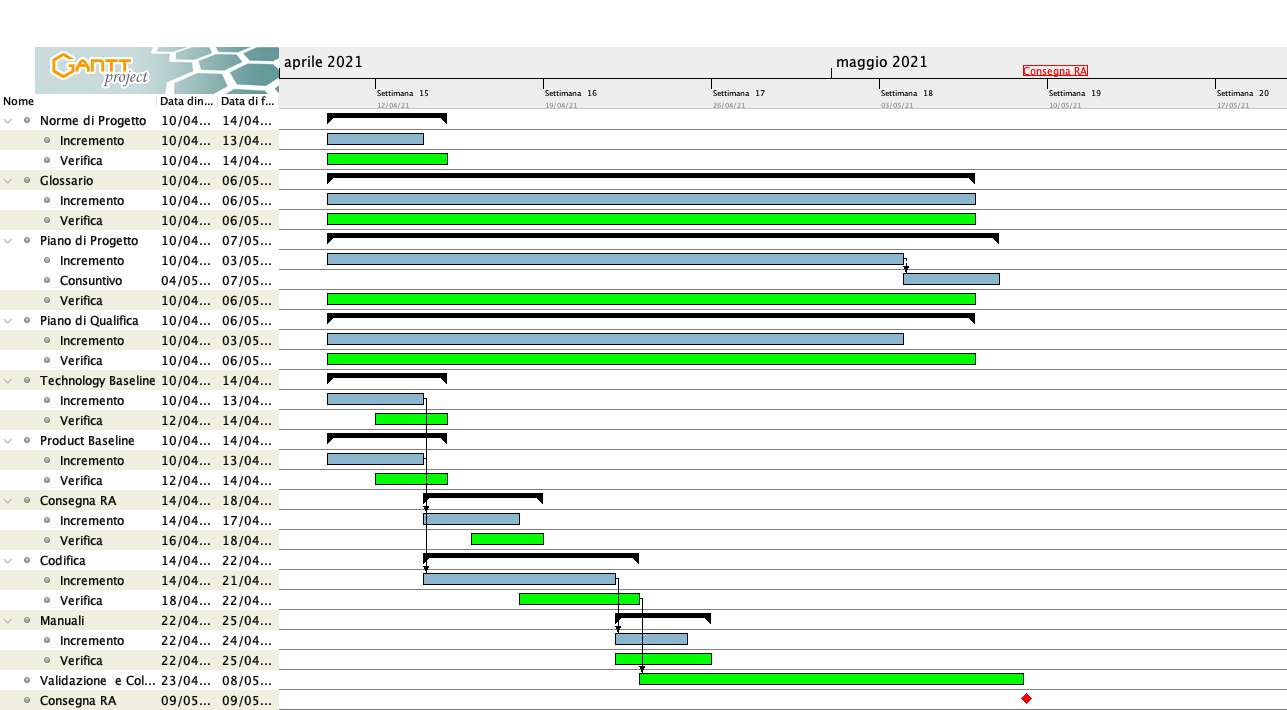
\includegraphics[width=\textwidth]{Immagini/GanttValidazioneECollaudo}
    \caption{Diagramma di Gantt dell'attività di validazione e collaudo}
\end{figure}